% ----------------------------------------------------------------------- %
% Arquivo: 04-Resultados.tex
% ----------------------------------------------------------------------- %
\chapter{Treinamento da Rede Neural para Detecção e localização de Defeitos em Placas de Circuito Impresso} \label{cap:treinamento}
%FALTA ESCERVER ESSA PARTE.
%Nesse capítulo serão discutidas a escolha e as etapas de preparação do \textit{dataset} para o treinamento, detalhes de configurações da rede neural utilizada e os resultados obtidos.

\section{Seleção da Rede Neural e do \textit{Framework} para o Treinamento} \label{cap:treinamento-rn}

Defeitos em placas de circuito impresso ocupam pequenas regiões da PCI, de forma que a proporção entre a área do objeto a ser detectado e a imagem inteira é muito pequena. Sendo assim, a escolha da rede neural deve considerar um bom desempenho para detecção de pequenos objetos. Segundo \citeonline{ref:Redmon-Farhadi}, a partir da versão três, a YOLO apresentou uma melhor performance para esse tipo de detecção, sendo recomendada para essa aplicação por \citeonline{ref:Valenti-et-al}, quando o tempo de treinamento não é tão relevante. Já a versão quatro da YOLO apresenta melhor desempenho para o treinamento em GPUs quando comparada a sua versão anterior.

Sendo assim, a rede neural escolhida para o treinamento da detecção de defeitos em PCIs foi a YOLO em sua quarta versão, proposta por \citeonline{ref:Bochkovskiy-Wang-Liao} em conjunto com \textit{framework} Darknet, que possui funções de cálculo das métricas de avaliação, desenho das caixas delimitadoras, entre outras.

\section{Seleção do Conjunto de Dados} \label{cap:treinamento-dataset}

Para a detecção e classificação de objetos, o conjunto de dados escolhido deve incluir além das imagens, a localização e classificação dos objetos de interesse.
O \textit{Dataset} escolhido para a detecção e localização de defeitos em PCIs é o \textit{HRIPCB: a challenging dataset for PCB defects detection and classification}, proposto por \citeonline{ref:Huang-et-al}.

As imagens das placas são capturadas por uma câmera do tipo industrial com dezesseis megapixel de resolução equipada com um sensor C-MOS \cite{ref:Huang-et-al}. O \textit{dataset} baseia-se em dez diferentes tipos de PCIs sem defeitos, conforme as imagens do \autoref{apendice:hripcb-pcbs} e, após a captura e ajustes, seis tipos de defeitos são adicionados manualmente em um \textit{software} de edição de imagens, onde cada imagem contém de dois a seis defeitos da mesma categoria em diferentes lugares da placa \cite{ref:Huang-et-al}. A distribuição dos defeitos está na \autoref{tab:treinamento-dataset}.

\begin{table}[!h]
\begin{center}
\caption{Distribuição dos defeitos no conjunto de dados HRIPCB.}
\label{tab:treinamento-dataset}
\begin{tabular}{ccc}
\toprule
\textbf{Tipo do Defeito} & \textbf{Número de Imagens} & \textbf{Quantidade Total de Defeitos} \\
\midrule \midrule
Falta de Estanho    & 115   & 497 \\
Falta de Cobre      & 115   & 492 \\
Circuito Aberto     & 116   & 482 \\
Curto-Circuito      & 116   & 491 \\
Excesso de Cobre    & 115   & 488 \\
Trilha Desconectada & 116   & 503 \\
\bottomrule
\end{tabular}
\indentedfont[0.96\textwidth]{\citeonline{ref:Huang-et-al}}
\end{center}
\end{table}

Para cada uma das imagens, existe um arquivo com extensão \textit{.xml} que mapeia as informações das caixas delimitadoras de cada defeito. Um exemplo desse arquivo está no \autoref{apendice:hripcb-xml}.
As anotações do HRIPCB não estão normalizadas e e são mapeadas em coordenadas cartesianas em pixeis $x_{min}$, $x_{max}$, que variam entre zero e a largura da imagem e $y_{min}$, $y_{max}$, que variam entre zero e a altura da imagem, conforme a \autoref{fig:resultados-hripcb-notacao}.

\begin{figure}[h!] %H
  \centering
  \caption{Anotações das caixas delimitadoras do \textit{dataset} HRIPCB.}
  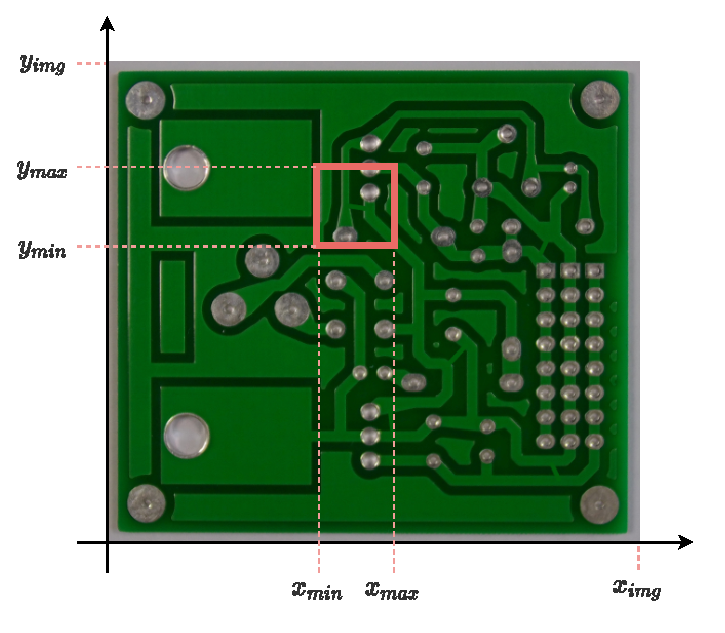
\includegraphics[scale=1]{img/img-resultados-hripcb-notacao.pdf}
  \label{fig:resultados-hripcb-notacao}
  \indentedfont[15.2cm]{Adaptado de \citeonline{ref:Huang-et-al}}
\end{figure}


A estrutura de arquivos do \textit{dataset} está na \autoref{fig:resultados-hripcb-estrutura}. Os arquivos dentro da pasta \textit{rotation} não foram utilizados já que não possuem as delimitações dos defeitos em arquivos de anotação.

\begin{figure}[h!] %H
  \centering
  \caption{Estrutura de arquivos do \textit{dataset} HRIPCB.}
  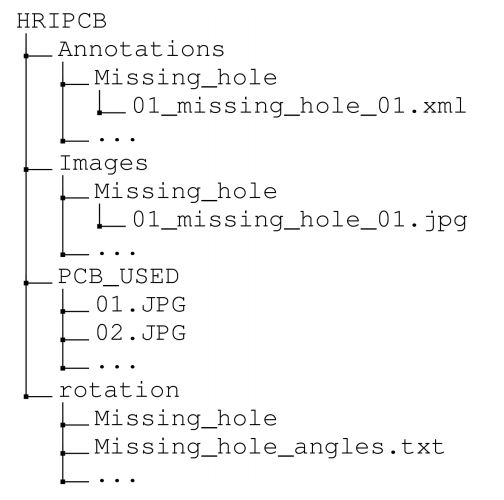
\includegraphics[scale=0.35]{img/img-resultados-hripcb-estrutura.png}
  \label{fig:resultados-hripcb-estrutura}
  \indentedfont[15.2cm]{\citeonline{ref:Huang-et-al}}
\end{figure}


\section{Configuração dos Arquivos para o Treinamento} \label{cap:treinamento-treinamento-config}

Para o treinamento, é necessário que os arquivos do \textit{dataset} escolhido estejam de acordo com o padrão utilizado pela YOLO e as imagens estejam separadas nos subconjuntos de teste e treinamento.

Os arquivos de anotação do \textit{dataset} HRIPC foram convertidos de \textit{.xml} para \textit{.txt} utilizando o \textit{script} em Python que está no \autoref{apendice:conversao}.
Esse \textit{script} percorre as pastas de anotação de cada defeito (\autoref{fig:resultados-hripcb-estrutura}), abrindo os arquivos \textit{.xml}, convertendo os dados conforme o padrão necessário para o treinamento e salvando esses dados em um arquivo de texto.

A conversão segue as Equações \ref{eq:resultados-conversao-x} e \ref{eq:resultados-conversao-y} para as coordenadas centrais $x_{center}$ e $y_{center}$ das caixas delimitadoras e as Equações \ref{eq:resultados-conversao-w} e \ref{eq:resultados-conversao-h} para a largura ($width$) e altura ($height$) das caixas delimitadoras, onde os resultados estão normalizados pela largura $x_{img}$ e altura  $y_{img}$ da imagem conforme indicado nos passos do \autoref{apendice:etapas-yolo}.

\begin{equation} \label{eq:resultados-conversao-x}
\mathrm{
  x_{center} = \frac{1}{x_{img}} \cdot ( x_{min} + \frac{x_{max} - x_{min}}{2})
}
\end{equation}

\begin{equation} \label{eq:resultados-conversao-y}
\mathrm{
  y_{center} = \frac{1}{y_{img}} \cdot ( y_{min} + \frac{y_{max} - y_{min}}{2})
}
\end{equation}

\begin{equation} \label{eq:resultados-conversao-w}
\mathrm{
  width = \frac{1}{x_{img}} \cdot (x_{max} - x_{min})
}
\end{equation}

\begin{equation} \label{eq:resultados-conversao-h}
\mathrm{
  height = \frac{1}{y_{img}} \cdot (y_{max} - y_{min})
}
\end{equation}

Além da conversão das coordenadas da caixa delimitadora, é necessário também especificar de maneira numérica qual é o defeito indicado por ela. Os defeitos estão numerados de acordo com a \autoref{tab:resultados-defeitos}.

\begin{table}[!h]
  \begin{center}
  \caption{Representação dos defeitos do conjunto de dados HRIPCB para o treinamento da Rede Neural.}
  \label{tab:resultados-defeitos}
  \begin{tabular}{cc}
    \toprule
    \textbf{Defeito} & \textbf{Representação Numérica}\\
    \midrule \midrule
    Circuito Aberto     & 1 \\
    Curto-Circuito      & 2 \\
    Falta de Cobre      & 3 \\
    Excesso de Cobre    & 4 \\
    Trilha Desconectada & 5 \\
    Falta de Estanho    & 6 \\
    \bottomrule
  \end{tabular}
  \indentedfont[0.96\textwidth]{Elaboração própria (2021)}
  \end{center}
\end{table}

O resultado da conversão do arquivo de anotação em \textit{.xml} do \autoref{apendice:hripcb-xml} está no \autoref{cod:conv}, onde cada linha representa um defeito suas coordenadas seguindo o padrão indicado por \citeonline{ref:Bochkovskiy} no \autoref{apendice:etapas-yolo}.

\lstinputlisting
[caption=Exemplo de arquivo de anotação para treinamento com YOLO.,
label=lst:hripcb,
firstnumber=1,
label=cod:conv]
{cod/anotacoes-HRIPCB.txt}

O \textit{dataset} foi dividido aleatoriamente nos sub-conjuntos treinamento e teste utilizando o \textit{script} do \autoref{apendice:divisao}, com 20\% dos arquivos para testes e o restante para o treinamento. Esse \textit{script} separa tanto as imagens quanto os arquivos de anotação e, além disso, também é responsável por criar os arquivos de texto \textit{train.txt} e \textit{test.txt} que lista todos os arquivos de cada subconjunto de treinamento e testes, respectivamente, necessários para o treinamento com YOLO.

O arquivo de configuração \textit{obj.data} é o apresendado no \autoref{cod:obj-data}. Esse arquivo contém o número de classes a serem treinadas além dos caminhos para os principais arquivos requeridos para o treinamento. O arquivo \textit{obj.names} está no \autoref{cod:obj-names} que lista todas as classes treinadas.

\lstinputlisting
[caption=Arquivo de configuração \textit{obj.data}.,
firstnumber=1,
label=cod:obj-data]
{cod/obj.data}

\lstinputlisting
[caption=Arquivo de configuração \textit{obj.names}.,
firstnumber=1,
label=cod:obj-names]
{cod/obj.names}

O arquivo de configuração das camadas da rede neural foi ajustado de acordo com o \autoref{apendice:etapas-yolo}. Sendo assim, o número máximo de \textit{batches} necessários para o treinamento foi $n_{classes} \cdot 2000 = 12000$ e a quantidade de filtros considerada foi de $(n_{classes} + 5) \cdot 3 = 33$.

\section{Treinamento} \label{cap:treinamento-treinamento}
O treinamento foi feito no Google Colaboratory, um ambiente que permite a execução de códigos Python em \textit{notebooks} Jupyter, adequado para Aprendizado de Máquina, análise de dados e educação, oferecendo recursos de computação como GPUs de forma gratuita \cite{ref:Colab}.

O código completo utilizado para o treinamento está disponível no \autoref{apendice:treinamento}, contendo todos os comandos utilizados.

O repositório do Darknet, disponibilizado \textit{online} por \citeonline{ref:Bochkovskiy} no endereço \url{https://github.com/AlexeyAB/darknet}, foi adicionado ao ambiente, por meio do comando \textit{git clone}. Além disso, foram manualmente adicionadas as pastas contendo os arquivos de configuração e do \textit{dataset} para o treinamento.

Alterações no arquivo \textit{makefile} foram feitas para que o treinamento ocorresse utilizando GPU (linhas quinze a dezessete do código do \autoref{apendice:treinamento}) e em seguida compilou-se o Darknet para o treinamento.

Com intuído de acelerar o treinamento, utilizou-se a transferência de aprendizado de forma que a rede foi inicializada com os pesos da \textit{yolov4.conv.137}, pré-treinada com um \textit{dataset} contendo mais de um milhão de imagens com objetos classificados em mais mil categorias \cite{ref:Redmon-et-al}. A transferência de aprendizado consiste em acelerar um novo treinamento a partir de resultados obtidos em treinamentos anteriores \cite{ref:Cai-Bileschi-Nielsen}.

\section{Resultados} \label{cap:treinamento-resultados}
O gráfico da \autoref{fig:resultados-grafico} mostra a evolução do desempenho durante o início do treinamento. Nota-se que para um pouco mais de mil e duzendos \textit{batches} a métrica de mAP, em vermelho, já estava com pico em 98\%. Da mesma forma, a função de perda, representada pelo traço azul, foi diminuindo consideravelmente conforme os pesos da rede neural se atualizavam. Esse gráfico não está completo pois é gerado pelo Darknet e salvo em um arquivo temporário e o treinamento foi interrompido em mil e quinhentos \textit{batches} e reiniciado a partir desse ponto.

\begin{figure}[h!] %H
  \centering
  \caption{Desempenho do início do treinamento da rede neural.}
  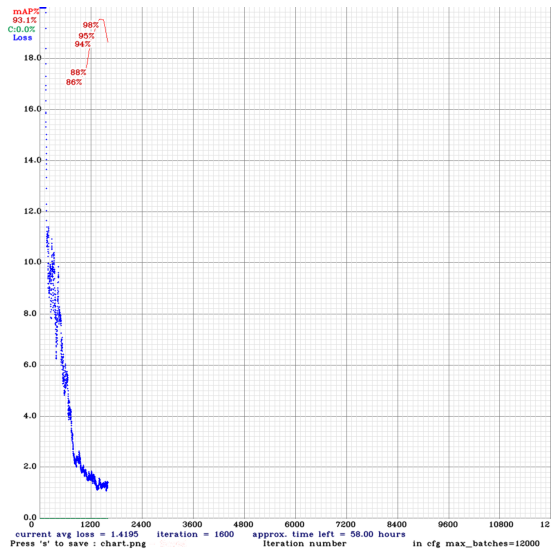
\includegraphics[scale=0.8]{img/img-resultados-grafico.png}
  \label{fig:resultados-grafico}
  \indentedfont[15.2cm]{Elaboração própria (2021)}
\end{figure}

As métricas de treinamento para os pesos obtidos são calculadas por meio do comando do Darknet presente no \autoref{cod:map}, onde o valor da \textit{flag thresh} indica o limiar de confiabilidade da predição utilizado para as métricas baseadas em matriz de confusão e a \textit{flag points} representa o tipo de aproximação para o cálculo da métrica de AP e mAP, onde o valor 0 quer dizer que não há nenhuma aproximação para o cálculo da área da curva precisão em função da sensibilidade.

\lstinputlisting
[caption=Comando Darknet para o cálculo das métricas de avaliação da rede neural.,
firstnumber=1,
label=cod:map]
{cod/darknet_map.txt}


O treinamento foi finalizado após dois mil e quinhentos \textit{batches}, já que os resultados  apresentavam bom desempenho, conforme a \autoref{tab:resultados-metricas}, que apresenta a métrica AP calculadas para cada uma das classes treinadas e a \autoref{tab:resultados-metricas-total}, que apresenta os resultados médios das classes treinadas. O tempo de treinamento não foi cronometrado, durando aproximadamente entre quinze e vinte horas.

\begin{table}[!h]
  \begin{center}
  \caption{Resultados de Precisão Média para as classes treinadas de defeitos em placas de circuito impresso.}
  \label{tab:resultados-metricas}
  \begin{tabular}{cccc}
    \toprule
    \textbf{Defeito} & \textbf{Precisão Média (AP)} \\
    \midrule \midrule
    Circuito Aberto     & 97,07\% \\
    Curto-Circuito      & 98,82\% \\
    Falta de Cobre      & 99,20\%  \\
    Excesso de Cobre    & 96,68\% \\
    Trilha Desconectada & 98,87\% \\
    Falta de Estanho    & 100,00\% \\
    \bottomrule
  \end{tabular}
  \indentedfont[0.96\textwidth]{Elaboração própria (2021)}
  \end{center}
\end{table}

\begin{table}[!h]
  \begin{center}
  \caption{Métricas de Avaliação para o conjunto das classes treinadas de defeitos em placas de circuito impresso, considerando um \textit{threshold} de confiabilidade da predição de 75\%.}
  \label{tab:resultados-metricas-total}
  \begin{tabular}{cccc}
    \toprule
    \textbf{Métrica} & \textbf{Resultado} \\
    \midrule \midrule
    Precisão            & 99,00\% \\
    Sensibilidade       & 94,00\% \\
    \textit{F1-score}   & 97,00\%  \\
    mAP                 & 98,44\% \\
    \bottomrule
  \end{tabular}
  \indentedfont[0.96\textwidth]{Elaboração própria (2021)}
  \end{center}
\end{table}

O gráfico de precisão em função da sensibilidade para cada uma das classes está na \autoref{fig:resultados-pr}. A \autoref{fig:resultados-pr-total} apresenta o mesmo gráfico considerando uma média de todas as classes para a curva de precisão em função da sensibilidade.
Esses gráficos foram construídos variando o valor de confiabilidade da predição (\textit{flag thresh}) dentro do intervalo $[0.001, 0.99]$ para as métricas de precisão e sensibilidade utilizando o comando do \autoref{cod:map}, além de alterar a função \textit{qsort} do arquivo ``detector.c'' que está localizado dentro da pasta \textit{Darknet/src/} e recompilar o Darknet para imprimir os valores de precisão e sensibilidade, já que sem isso apenas a métrica de AP é apresentada para cada classe.


\begin{figure}[H] %H
  \centering
  \caption{Curvas de precisão em função da sensibilidade para cada classe treinada.}
  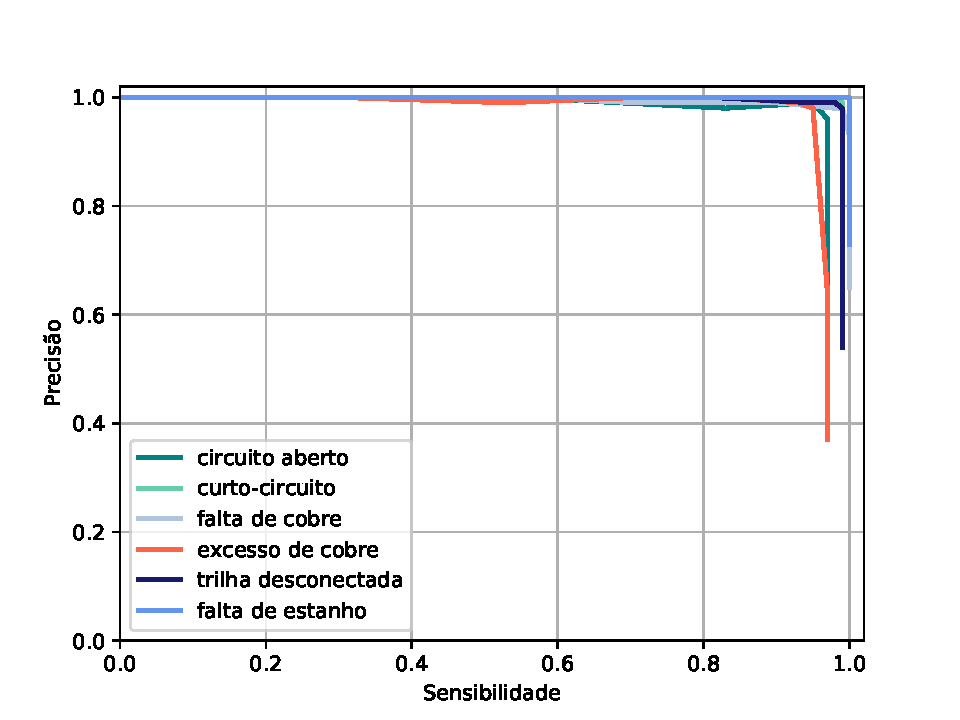
\includegraphics[scale=0.8]{img/img-resultados-pr.pdf}
  \label{fig:resultados-pr}
  \indentedfont[15.2cm]{Elaboração própria (2021)}
\end{figure}

\begin{figure}[H] %H
  \centering
  \caption{Curva de precisão em função da sensibilidade para o conjunto de classes treinado.}
  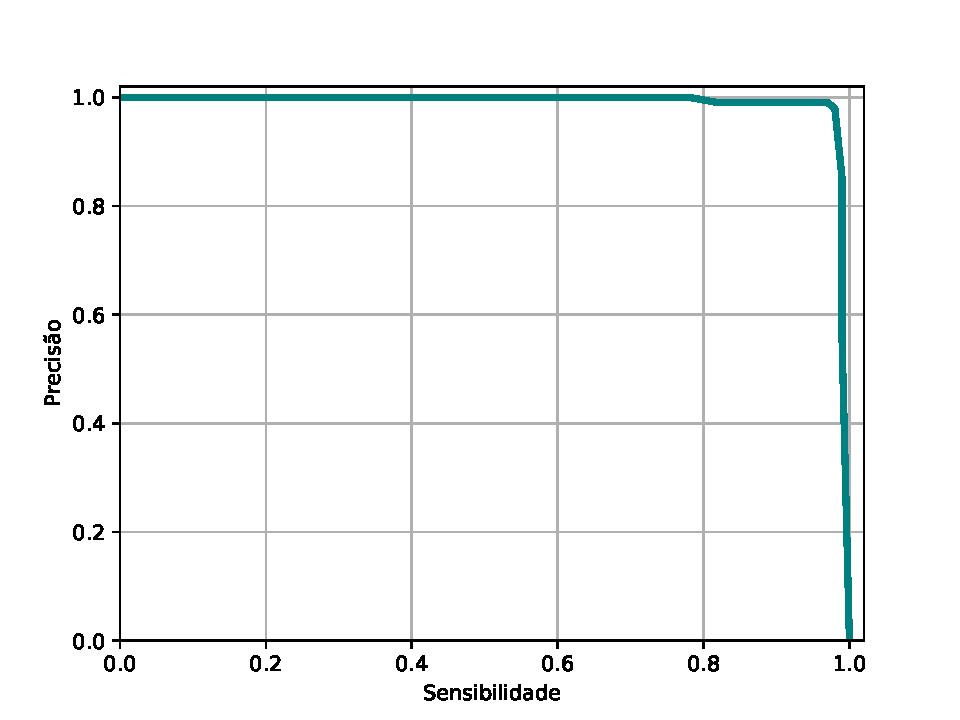
\includegraphics[scale=0.8]{img/img-resultados-pr-total.pdf}
  \label{fig:resultados-pr-total}
  \indentedfont[15.2cm]{Elaboração própria (2021)}
\end{figure}

As Figuras \ref{fig:resultados-predicao-1}, \ref{fig:resultados-predicao-2} e \ref{fig:resultados-predicao-3} apresentam resultados de detecção para imagens com defeitos variados adicionados manualmente em \textit{software} de edição de imagem a partir de PCIs do \textit{dataset} sem presença de defeitos.
Essas imagens baseiam-se nas apresentadas no \autoref{apendice:hripcb-pcbs}. O número indicado ao lado do nome do defeito significa a confiabilidade da predição, onde 1 indicaria uma predição 100\% confiável.

\begin{figure}[H] %H
  \centering
  \caption{Resultado de predição para imagem com defeito, teste 1.}
  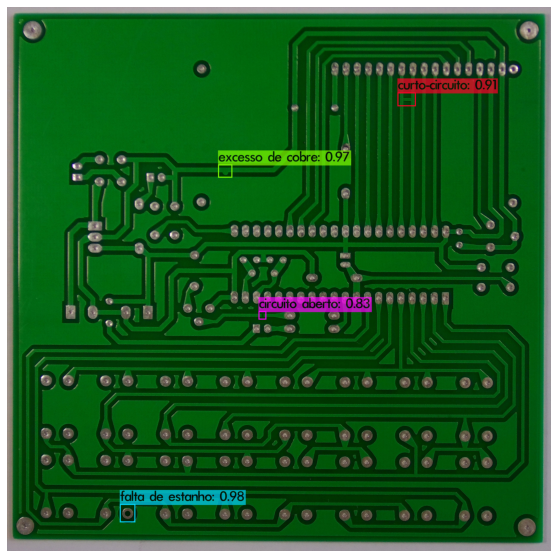
\includegraphics[scale=0.5]{img/img-resultados-predicao-1.jpg}
  \label{fig:resultados-predicao-1}
  \indentedfont[15.2cm]{Adaptado de \citeonline{ref:Huang-et-al}}
\end{figure}

\begin{figure}[H] %H
  \centering
  \caption{Resultado de predição para imagem com defeito, teste 2.}
  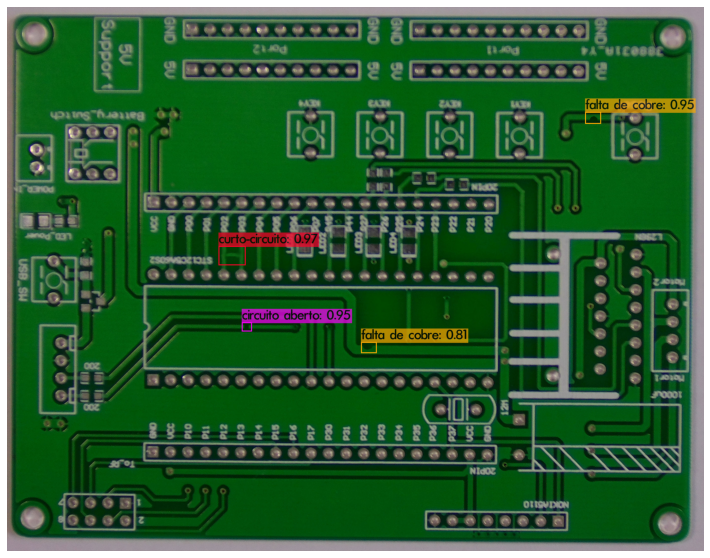
\includegraphics[scale=0.5]{img/img-resultados-predicao-2.jpg}
  \label{fig:resultados-predicao-2}
  \indentedfont[15.2cm]{Adaptado de \citeonline{ref:Huang-et-al}}
\end{figure}

\begin{figure}[!h] %H
  \centering
  \caption{Resultado de predição para imagem com defeito, teste 3.}
  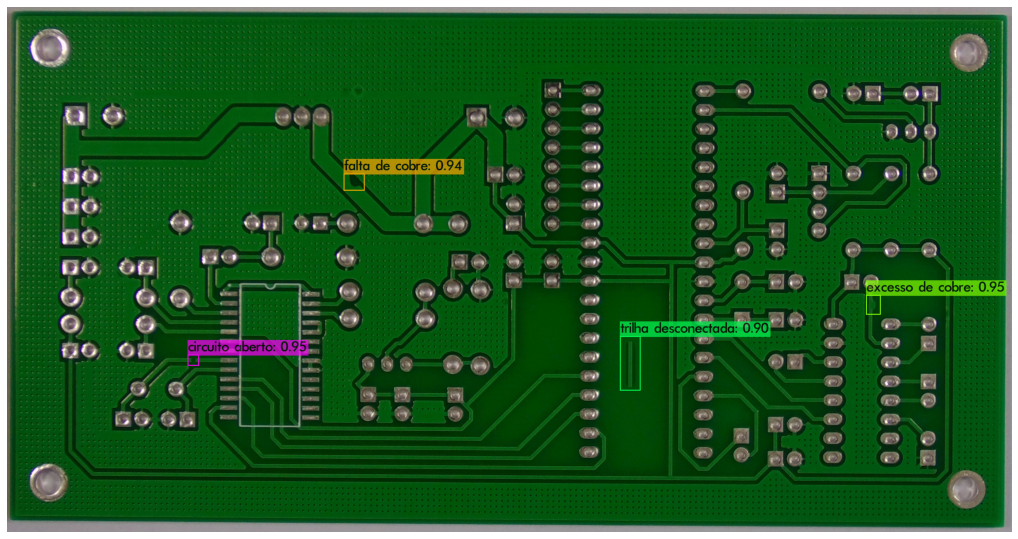
\includegraphics[scale=0.45]{img/img-resultados-predicao-3.jpg}
  \label{fig:resultados-predicao-3}
  \indentedfont[15.2cm]{Adaptado de \citeonline{ref:Huang-et-al}}
\end{figure}

As Figuras \ref{fig:resultados-predicao-ruim-1} e \ref{fig:resultados-predicao-ruim-2} apresentam resultados de detecção para imagens de fora do \textit{dataset}. Em ambas figuras, as setas indicam os defeitos que não foram detectados pela rede neural.
A \autoref{fig:resultados-predicao-ruim-2} aponta os furos de vias como defeitos, já que o \textit{dataset} utilizado considera vias ou furos sem a cobertura de estanho como um defeito.

\begin{figure}[H] %H
  \centering
  \caption{Resultado de predição para imagem com defeito, teste 4.}
  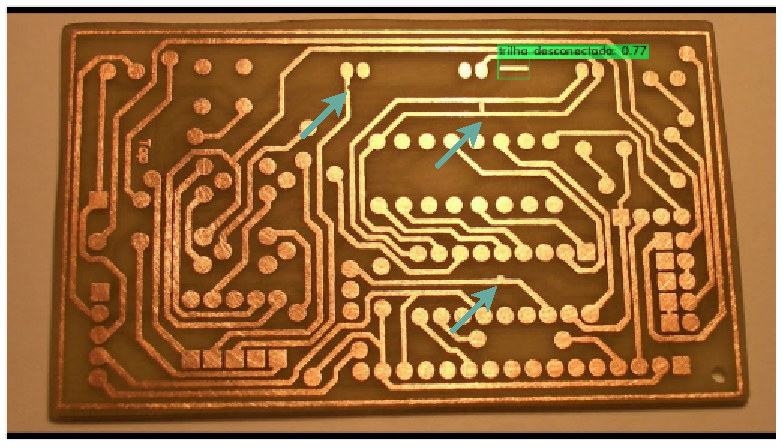
\includegraphics[scale=0.95]{img/img-resultados-predicao-ruim-1.pdf}
  \label{fig:resultados-predicao-ruim-1}
  \indentedfont[15.2cm]{Adaptado de \citeonline{ref:Khambhala}}
\end{figure}

\begin{figure}[!h] %H
  \centering
  \caption{Resultado de predição para imagem com defeito, teste 5.}
  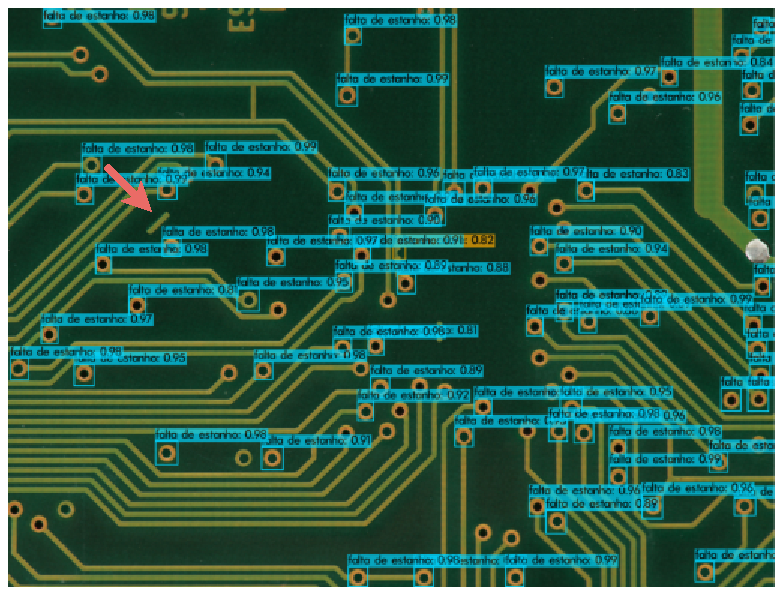
\includegraphics[scale=0.95]{img/img-resultados-predicao-ruim-2.pdf}
  \label{fig:resultados-predicao-ruim-2}
  \indentedfont[15.2cm]{Adaptado de \citeonline{ref:Dratza}}
\end{figure}

\chapter{Interface de Aplicação} \label{cap:api}
Para demonstração dos resultados obtidos com o treinamento da rede neural, uma aplicação \textit{web} foi implementada utilizando Flask, um \textit{framework} de fácil uso que possibilita a integração com outros módulos Python.

O código desenvolvido está disponível no repositório online \url{https://github.com/anabdck/pcb-defect-detection-api} e as etapas de instalação e configuração estão no \autoref{apendice:conf-api}.

%\section{Estrutura} \label{cap:api-estrutura}
A estrutura da aplicação foi construída de acordo com o apresentado na \autoref{fig:resultados-api-estrutura}.

\begin{figure}[!h] %H
  \centering
  \caption{Estrutura da interface de aplicação proposta.}
  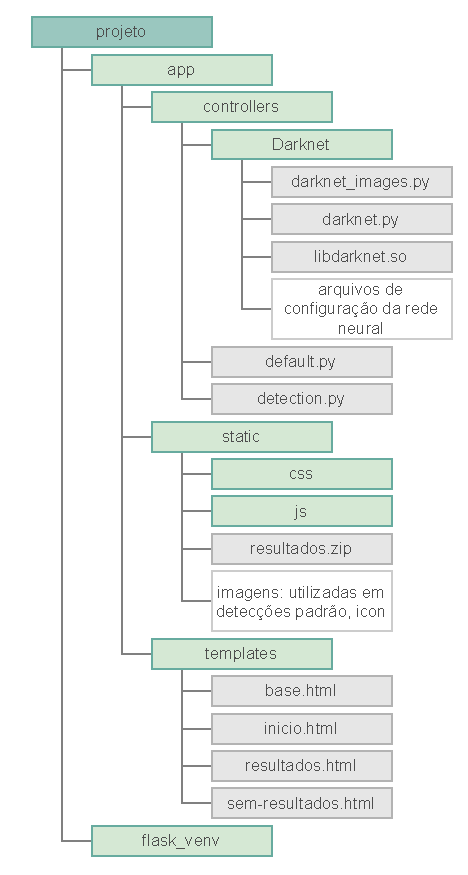
\includegraphics[scale=1.05]{img/img-resultados-api-estrutura.pdf}
  \label{fig:resultados-api-estrutura}
  \indentedfont[15.2cm]{Elaboração própria (2021)}
\end{figure}

As páginas \textit{web} apresentadas ao usuário utilizam HTML5, CSS3, Java Script e Bootstrap, organizadas dentro das pastas \textit{static} e \textit{templates} e o roteamento das páginas ocorre em \textit{default.py} dentro da pasta \textit{controllers}.

O módulo de detecção \textit{detection.py} é responsável por invocar o Darknet e processar a imagem para a detecção dos defeitos utilizando os arquivos de configuração da rede neural e os pesos treinados.
Para isso, é necessária a biblioteca \textit{libdarknet.so}, compilada para o servidor utilizado conforme o indicado nos passos do
\autoref{apendice:conf-api}.

O Fluxograma da \autoref{fig:resultados-api-etapas} apresenta de maneira abreviada as etapas de detecção dos defeitos, indicando o momento em que as diferentes páginas são renderizadas e quais são os endereços que foram roteados para a aplicação utilizados no processo.

\begin{figure}[H] %H
  \centering
  \caption{Fluxograma da detecção de defeitos de placas de circuito impresso dentro da interface de aplicação proposta.}
  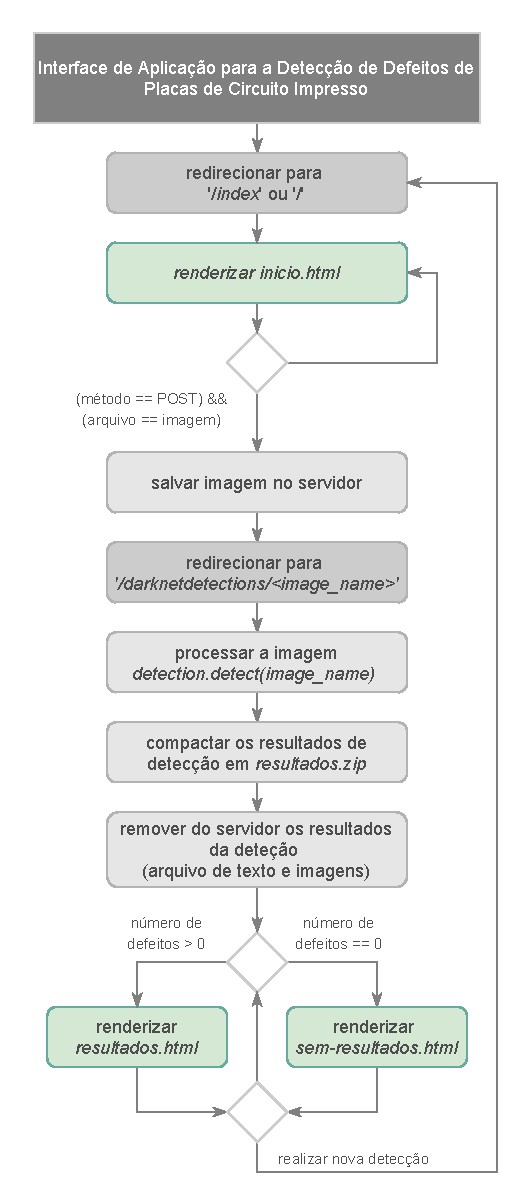
\includegraphics[scale=1.03]{img/img-resultados-api-fluxograma.pdf}
  \label{fig:resultados-api-etapas}
  \indentedfont[15.2cm]{Elaboração própria (2021)}
\end{figure}

O endereço inicial apresenta a tela da \autoref{fig:resultados-api-1}, onde o usuário pode fazer o \textit{upload} de uma imagem para a detecção ou, ao rolar a página para baixo, pode escolher uma das quatro imagens que já estão no servidor para a detecção, conforme a tela da \autoref{fig:resultados-api-2}. É possível fazer apenas o \textit{upload} de arquivos de imagens com extensões \textit{png},\textit{jpg} ou \textit{jpeg}. Caso seja feito o \textit{upload} de outros tipos de arquivos, é feito o redirecionamento para a página inicial novamente, já que as demais extensões não são aceitas pela rede neural.

Se arquivo escolhido for de uma das extensões permitidas ou o usuário escolher uma das imagens que está no servidor, a detecção dos defeitos é feita. Se a rede neural encontrar defeitos na imagem, a tela da \autoref{fig:resultados-api-3} é apresentada ao usuário, onde a indicação dos defeitos encontrados é feita por meio das caixas delimitadoras resultantes impressas na imagem processada. Uma mensagem indicando o tempo de processamento e a quantidade de defeitos encontrados é exibido ao usuário. O botão de ``\textit{Download} dos Resultados'' salva no computador do usuário um arquivo compactado contendo a imagem com as caixas delimitadoras e um arquivo de texto de anotação no padrão YOLO. Caso nenhum defeito é encontrado, a imagem original é mostrada ao usuário, além do aviso indicando o tempo de processamento, conforme a \autoref{fig:resultados-api-5}. O botão de ``\textit{Download} dos Resultados'' fica travado nesse caso.

\begin{landscape}
  \begin{figure}[H] %H
    \centering
    \caption{Tela Inicial 1 da Interface de Aplicação.}
    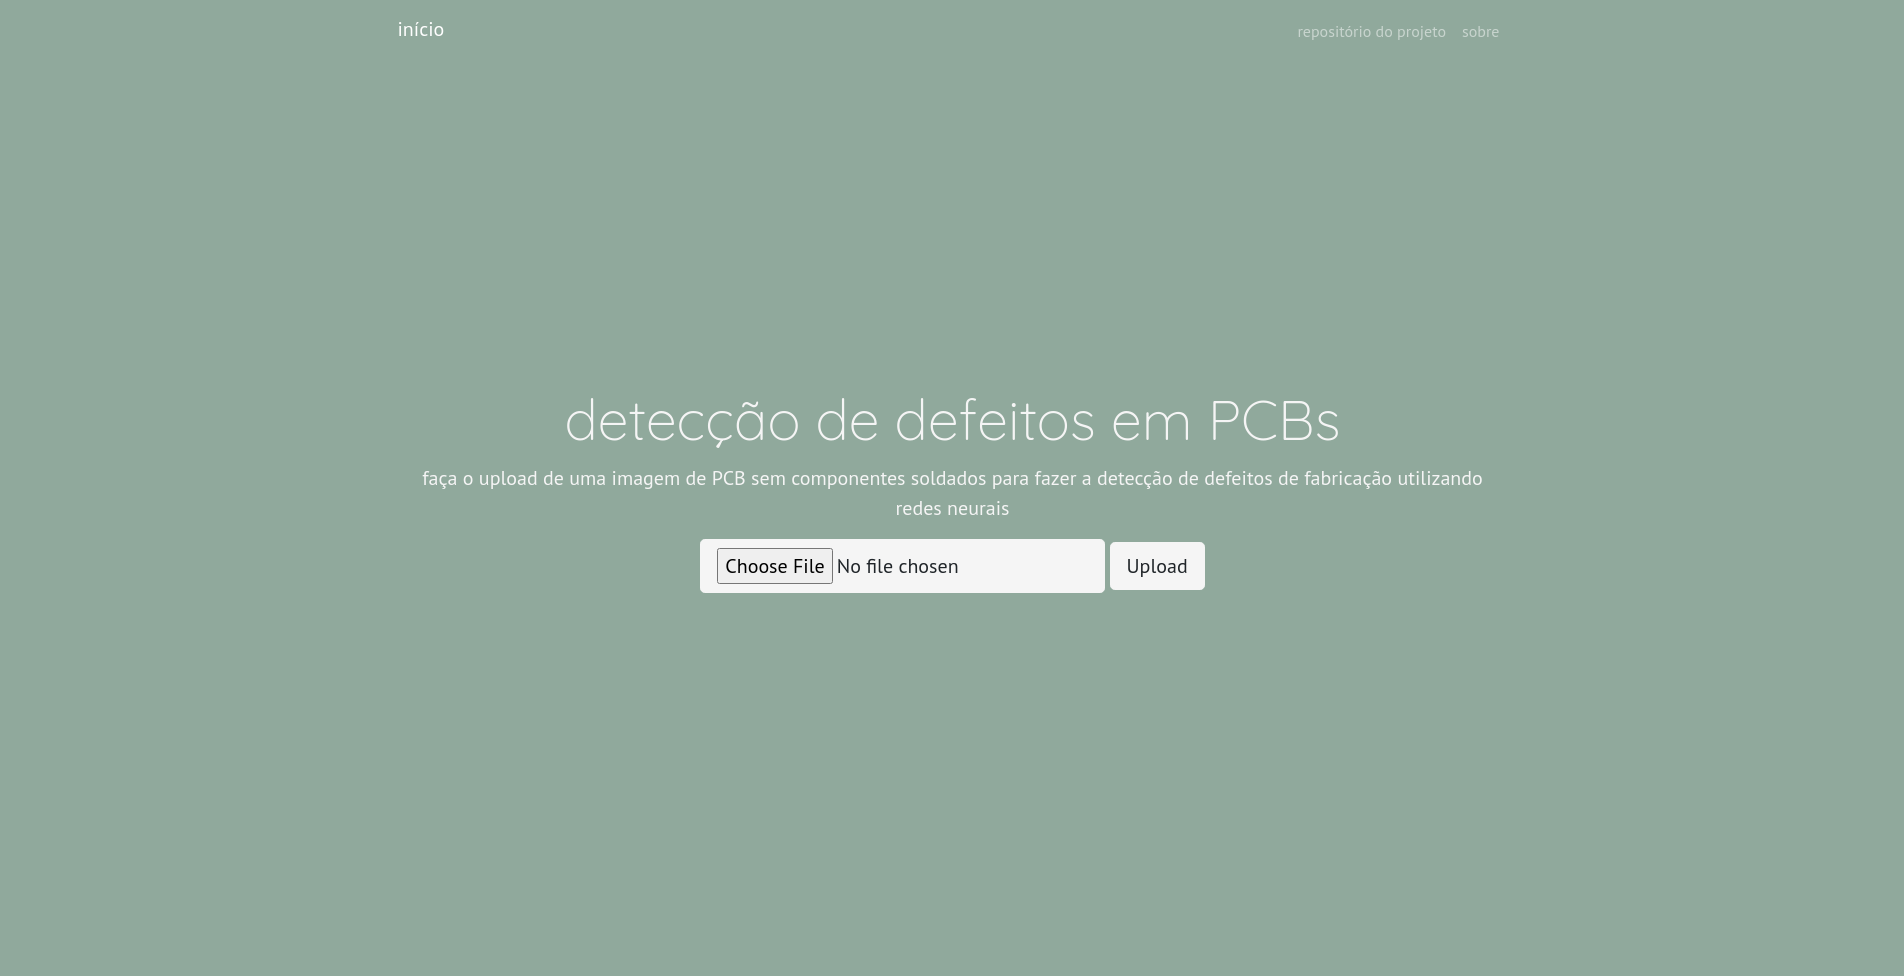
\includegraphics[scale=0.36]{img/api/1.png}
    \label{fig:resultados-api-1}
    \indentedfont[15.2cm]{Elaboração própria (2021)}
  \end{figure}
\end{landscape}

\begin{landscape}
  \begin{figure}[H] %H
    \centering
    \caption{Tela Inicial 2 da Interface de Aplicação.}
    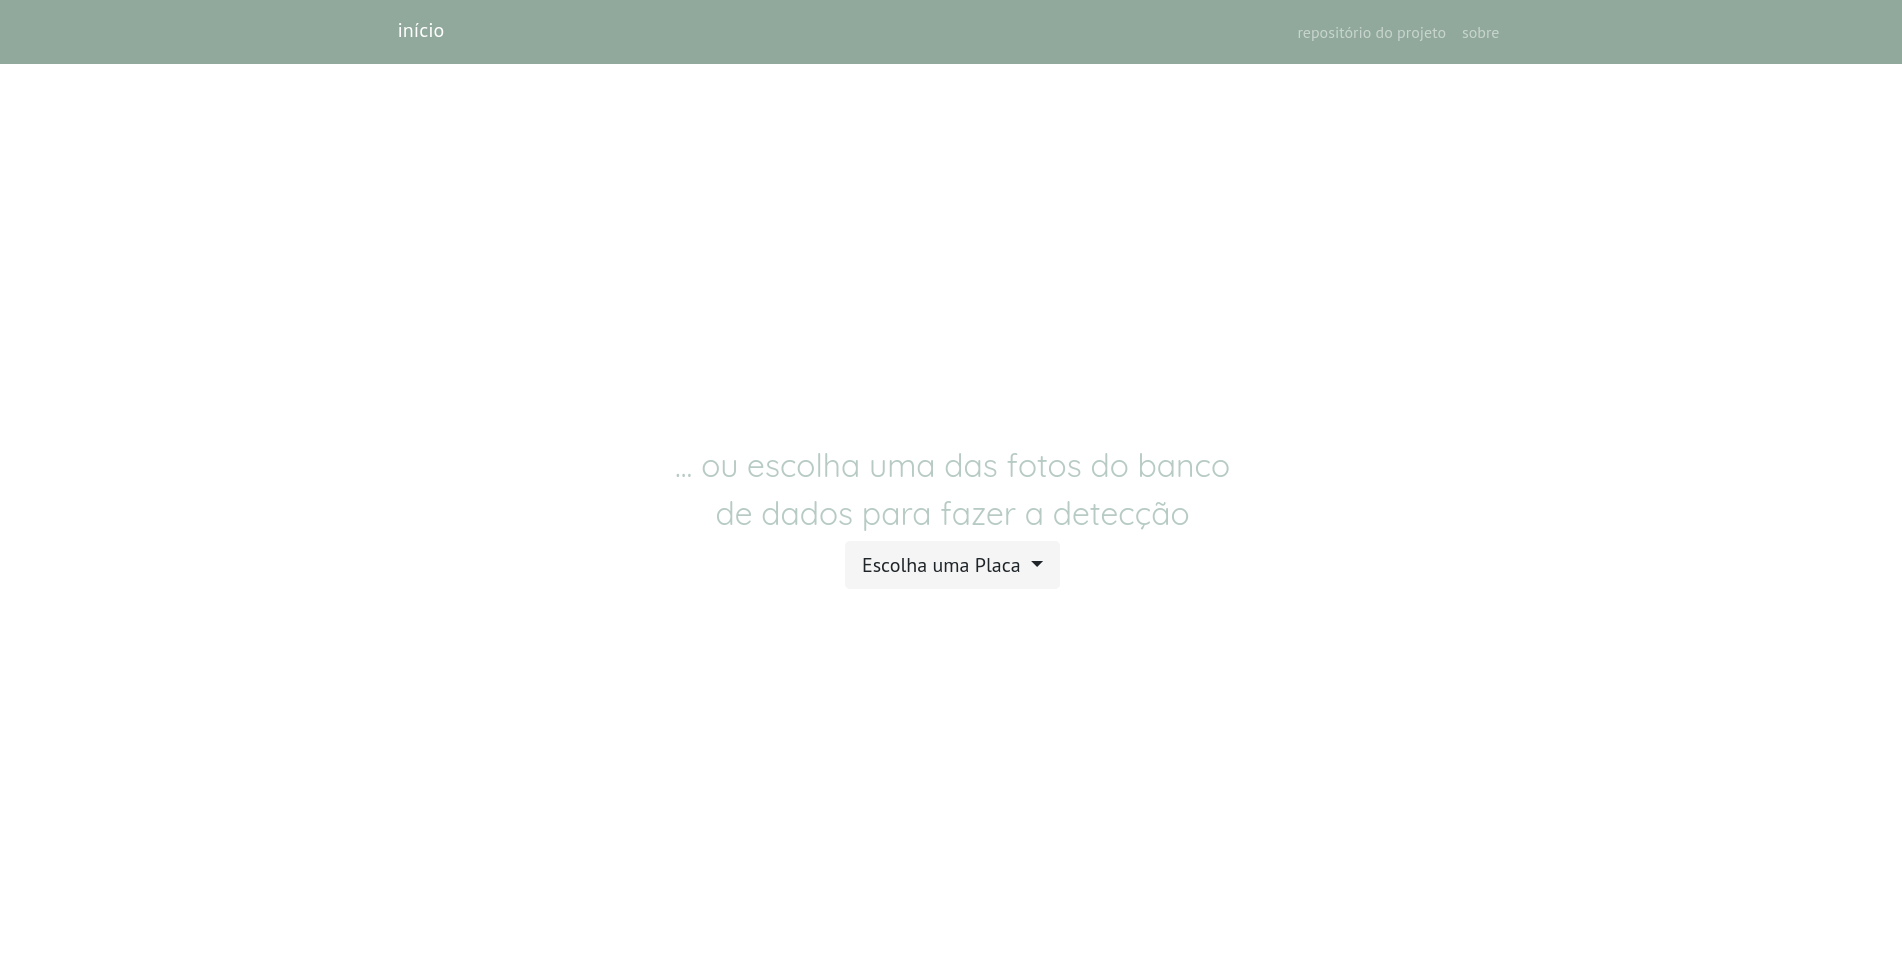
\includegraphics[scale=0.36]{img/api/2.png}
    \label{fig:resultados-api-2}
    \indentedfont[15.2cm]{Elaboração própria (2021)}
  \end{figure}
\end{landscape}

\begin{landscape}
  \begin{figure}[H] %H
    \centering
    \caption{Tela da Interface de Aplicação para imagem com detecções.}
    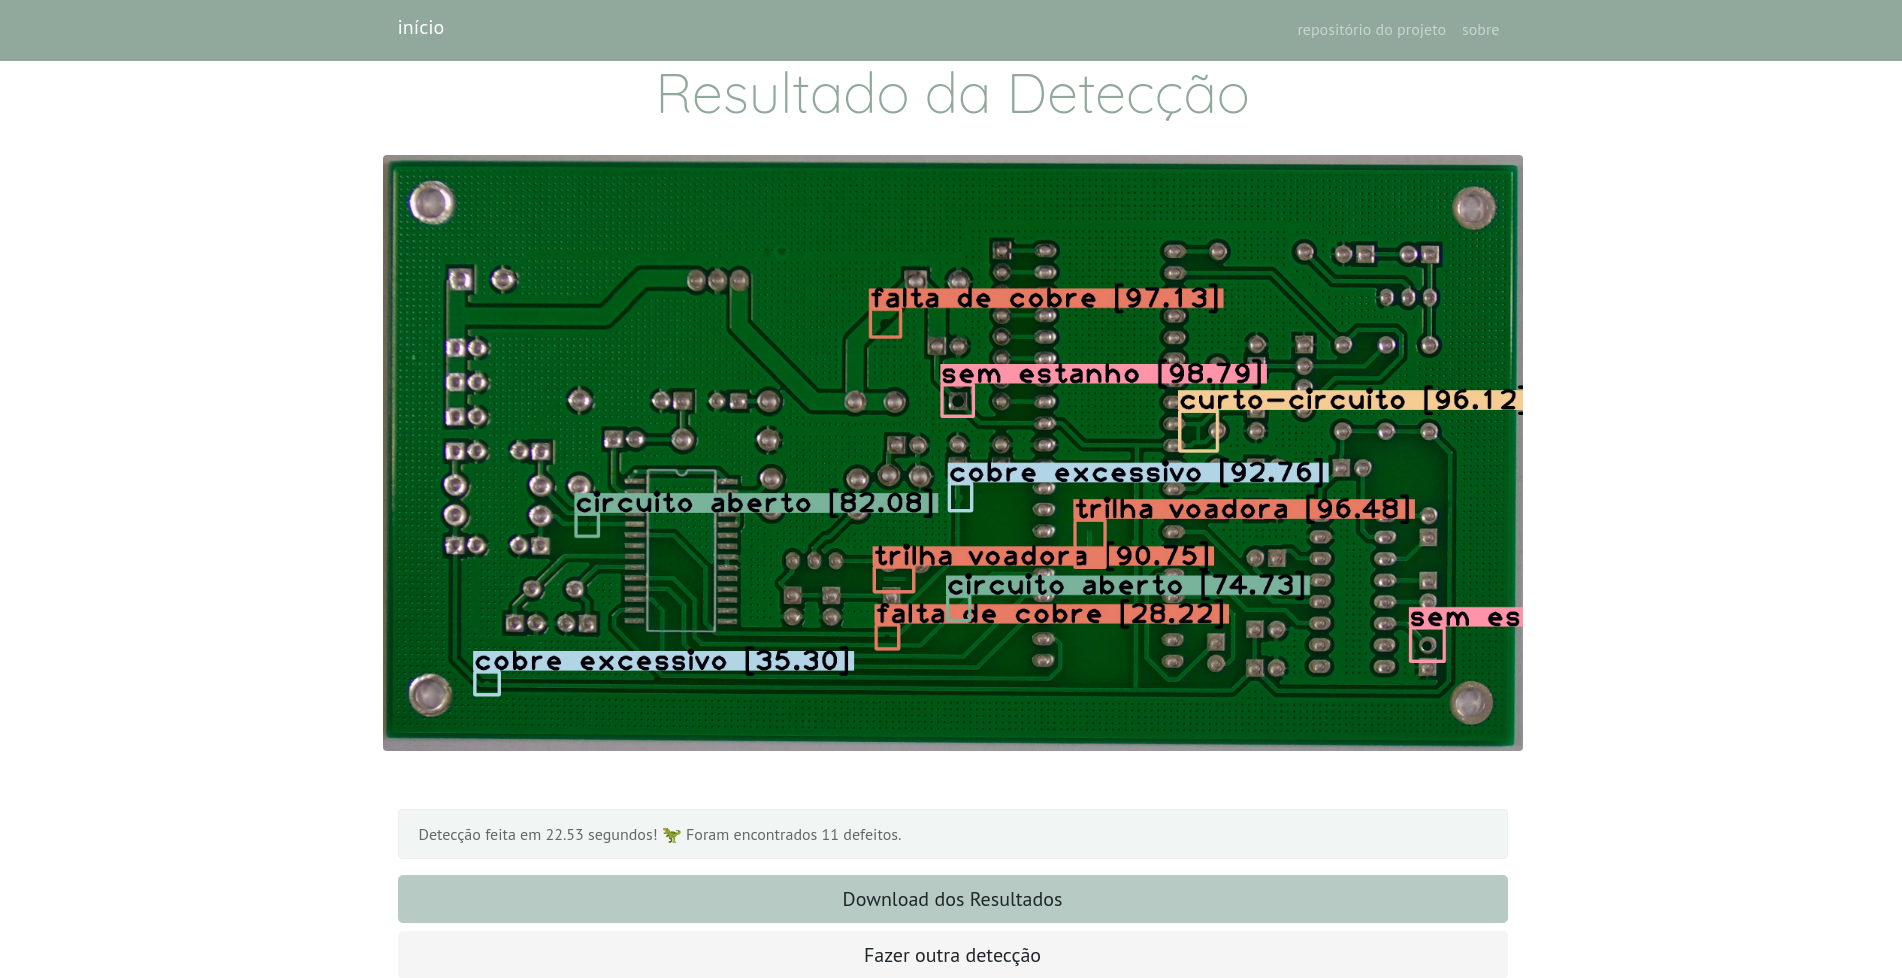
\includegraphics[scale=0.36]{img/api/3.png}
    \label{fig:resultados-api-3}
    \indentedfont[15.2cm]{Elaboração própria (2021)}
  \end{figure}
\end{landscape}

\begin{landscape}
  \begin{figure}[H] %H
    \centering
    \caption{Tela da Interface de Aplicação para imagem sem detecções.}
    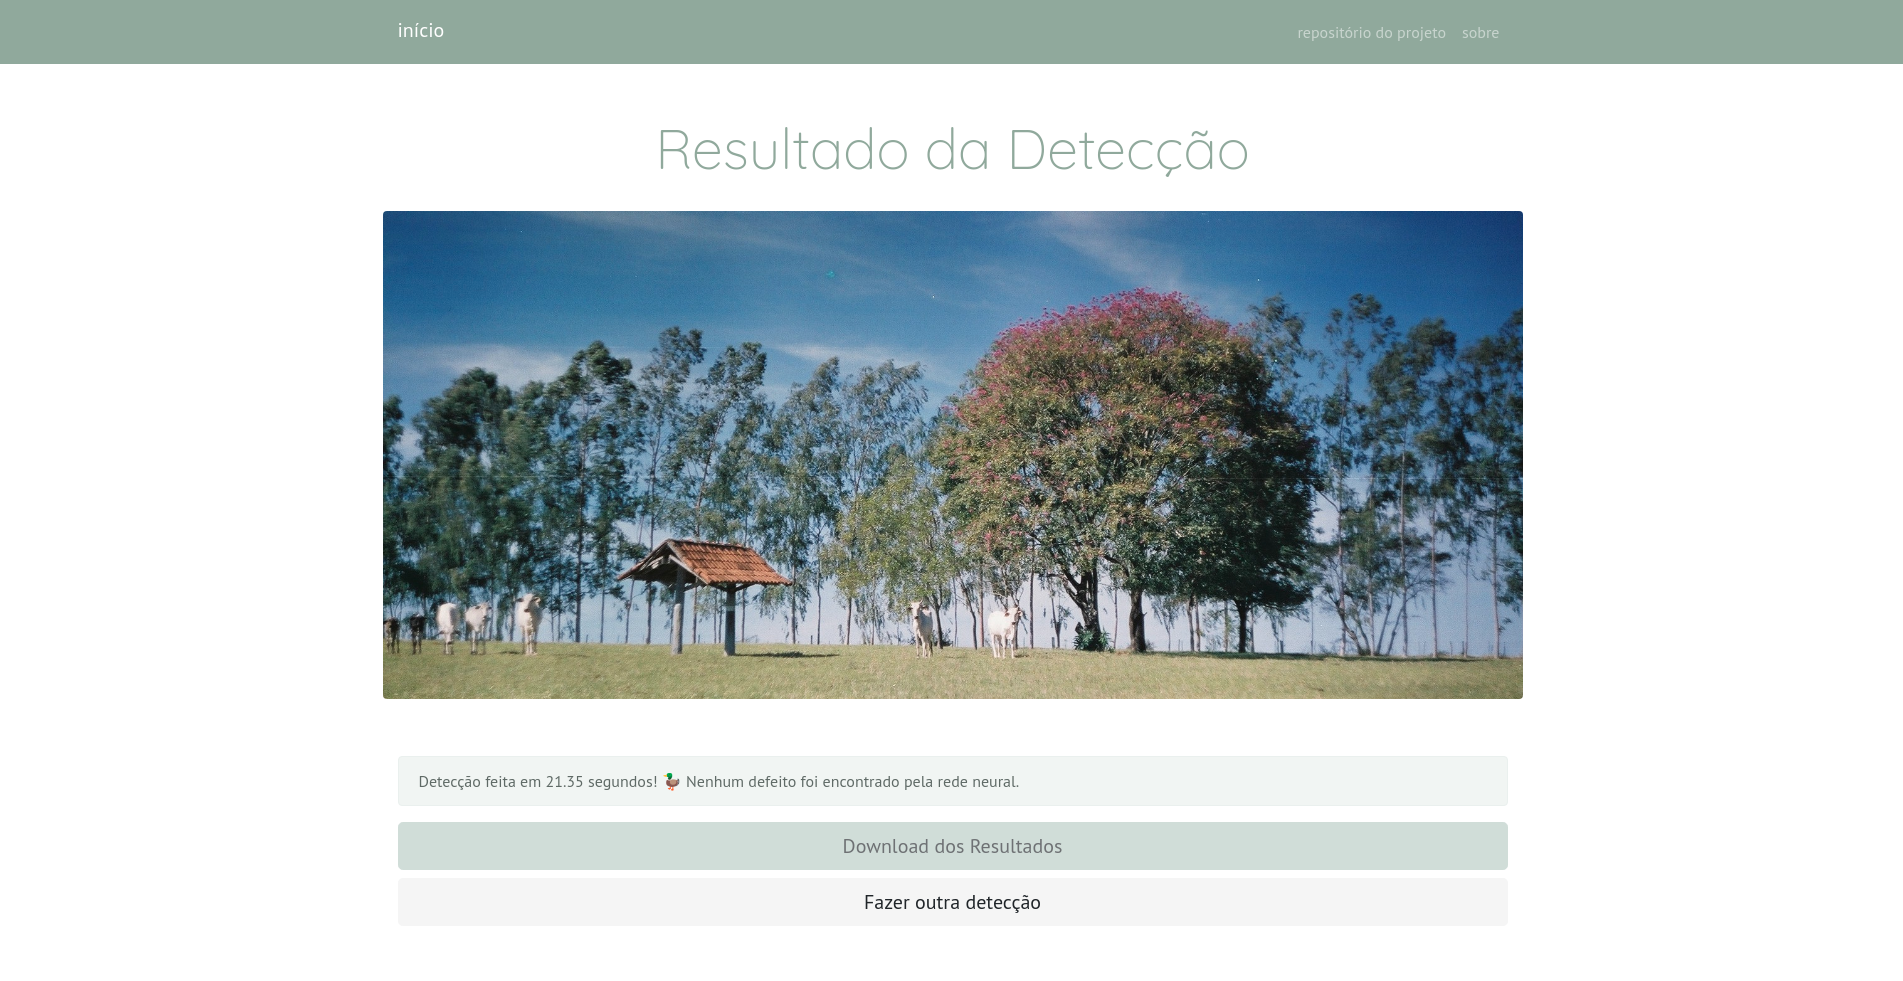
\includegraphics[scale=0.36]{img/api/5.png}
    \label{fig:resultados-api-5}
    \indentedfont[15.2cm]{Elaboração própria (2021)}
  \end{figure}
\end{landscape}
